\documentclass[a4paper,fleqn]{cas-dc}
\usepackage[numbers,sort&compress]{natbib}
\usepackage{amsmath,amssymb,booktabs,microtype}
\usepackage{graphicx,xr,xurl}
\hypersetup{pdfauthor={Meshaal Mouawad},pdfsubject={Half-moon classification and representation loss},pdfcreator={LaTeX3; cas-dc.cls; hyperref.sty}}
\externaldocument{Supplement_labels}
\graphicspath{{../Figures/}}
\newcommand{\R}{\mathbb R}
% Use the publisher's nologo title option to keep the submission source flat.
\ExplSyntaxOn
\keys_set:nn { stm / mktitle } { nologo = true }
\ExplSyntaxOff
% V10: connected journal-first research argument and selective mathematical notation.
\newcommand{\HalfMoonIntroduction}{%
\section{Introduction}\label{sec:introduction}
Normalizing observations to unit length suppresses differences in scale by retaining direction and discarding distance from a chosen origin. If that distance helps distinguish classes, observations requiring different labels can become identical before a classifier sees them. We investigate whether choosing a different origin can prevent this loss and how little distance information must be restored when it cannot. Geometric proofs and controlled neural experiments connect the retained information to the smallest achievable classification error.

The half-moon problem makes this difficulty visible. Each observation is a point labeled by which of two crescent-shaped regions generated it (Fig.~\ref{fig:geometry}). Two points on the same ray share a direction even when their labels differ. Moving the origin changes which points merge, making centering part of the information-preservation problem. We measure the effect through Bayes risk, the smallest population classification error attainable from a given representation. This separates information discarded by preprocessing from additional error introduced by learning.

Recent \emph{Pattern Recognition Letters} research approaches this distinction from complementary directions. Poblete et al.\ \citep{Poblete2026} hold learned representations fixed and show that classifier rankings vary with the dataset. Ahmadian and Lindsten\ \citep{Ahmadian2025} observe poorer novelty-detection performance after unit normalization and suggest that lost radial information contributes. These findings motivate asking what the representation itself makes possible. Decision-sufficiency and lossless-transformation theory already characterize preservation of optimal decisions \citep{Silva2012,Silva2024,Gyorfi2023}; the geometric question is how that preservation behaves as the normalization origin changes over the whole plane.

A positive error at each tested origin does not establish a positive lower bound across all origins: increasingly distant centers might still make the loss arbitrarily small. We resolve this issue by proving a uniform limit to orthogonal-projection risk as origins recede. Connected planar regions favoring opposite decisions then yield a global loss criterion and computable lower certificates. For a specified half-moon family, these results establish unavoidable loss in both disjoint and overlapping configurations. In one disjoint midpoint configuration, a single near/far radius measurement selects between two angular rules and restores every class decision. Its exact operating interval determines the permissible radius-measurement error. Paired neural studies compare learned errors with these representation-specific limits.
}

\newcommand{\HalfMoonBackground}{%
\section{Background and related work}\label{sec:background}
\paragraph{What direction retains.}
The spatial-sign transformation retains the direction of a centered observation \citep{Serneels2006}. For an observation $x$ and shared origin $c$, it is $T_c(x)=(x-c)/\|x-c\|$ when $x\ne c$. For illustration, $(1,1)$ and $(2,2)$ become identical about $(0,0)$; about $(0,1)$ their directions differ. Keeping the radius $\rho=\|x-c\|$ alongside direction $u$ permits reconstruction through $x=c+\rho u$. This gives a full-information control against which to assess discarding radius.

\paragraph{Geometric evidence in recent classification research.}
Poblete et al.\ \citep{Poblete2026} compare four classifiers on the same fixed feature vectors from trained generative models across eight datasets. Their class-centered radial-compatibility descriptor measures direction-independent spread within classes and radial separation between classes. Classifier rankings vary, and the predicted directional association between this descriptor and classifier advantage is unsupported. This separates a useful description of geometry from a guaranteed decision rule. Our question instead concerns how moving a shared normalization origin changes the observations that become indistinguishable.

Ahmadian and Lindsten\ \citep{Ahmadian2025} combine radial scoring with context quantization for human-activity novelty detection. Their separate normalization and quantization ablations show that the normalized variant performs worse than the unnormalized radial-kernel variant without quantization on both principal datasets. They suggest information loss under normalization as an explanation. Yang et al.\ \citep{Yang2026Compression} examine another consequence of compression: image-classification predictions can remain correct while visual explanations deteriorate, motivating an explanation-aware training objective. Together, these studies show why retained task information must be specified explicitly. Here the object is the optimal class decision after a fixed direction map, before classifier fitting.

\paragraph{Preserved decisions and restricted radial recovery.}
The Bayes decision selects the more probable class at an input. Silva and Narayanan\ \citep{Silva2012} analyze representation-induced error; Silva et al.\ \citep{Silva2024} distinguish retaining information about the label from retaining the optimal decision. Gy\"orfi et al.\ \citep{Gyorfi2023} characterize losslessness across loss functions through conditional independence and derive excess-risk upper bounds. Encoder--decoder analysis also relates information loss to prediction losses \citep{Silva2025}. These results establish the statistical target; a direction map requires a geometric account of which opposing decisions it merges.

Dubois et al.\ \citep{Dubois2021} characterize compression for invariant predictive tasks and identify unit direction as a maximal invariant for scaling: it gives the same encoding precisely to points on the same ray. Their task condition requires the conditional label law to be constant within each equivalence class. Oppositely labeled points on a shared ray expose precisely the condition that direction-only compression can violate. 

Oehler and Gray\ \citep{OehlerGray1995} incorporate Bayes risk into vector quantization. {\c S}enozan and Soylu\ \citep{Senozan2024} learn entropy-based attribute cut points that accommodate non-monotonic class relationships. Our repair restricts the extra measurement to one common-threshold radius bit and proves its sufficiency, operating interval and error tolerance. Ni et al.\ \citep{Ni2024} study finite-sample classification capacity through repeated affine transformations and normalization, providing a different guarantee from recovery over continuous class regions.

Magnitude retention in attention \citep{Meng2026}, decision-aware logit normalization \citep{Ding2026}, learned graph centering \citep{Scholkemper2025} and adaptive input transformation \citep{September2024} offer mechanisms for controlling retained information. Spatial-sign discriminants use class locations to classify unnormalized observations \citep{Zhuang2026}; their quadratic extension estimates interclass scale \citep{Shen2025}. The present analysis holds the population and direction transformation explicit so that a radial measurement's contribution can be proved separately from learning.

\paragraph{From a chosen projection to every origin.}
Hamsici and Martinez\ \citep{Hamsici2008} optimize projected Bayes error for Gaussian classes with common covariance. Oh\ \citep{Oh2025} addresses merging of nearby classes under linear dimensionality reduction by optimizing generalized means of pairwise scatter ratios, with classification experiments on five datasets. Spherical-model analysis compares decision boundaries with Gaussian approximations \citep{Hamsici2007}, and normalized-feature support vector machines adjust decision offsets \citep{Graf2003}. These approaches clarify the relationship between a chosen representation and its class separation. Our optimization variable is the common origin of a nonlinear radial map.

Hurtado et al.\ \citep{Hurtado2001} study wedge separation of finite planar point sets. Their convex-hull obstruction motivates a continuous-population construction in which shared rays carry opposing probability mass. Orthogonal projections are the geometric limits of radial projections from distant origins \citep{Orponen2019}. Combining these streams identifies the remaining question: when does loss at every finite origin remain bounded away from zero even as the origin escapes to infinity, and what restricted radial measurement restores the decision? The uniform risk limit, signed-density certificates and explicit one-bit decoder provide the corresponding analytical answers.
}

\newcommand{\HalfMoonDiscussion}{%
\section{Discussion}\label{sec:discussion}
The global criterion explains why searching for a better origin can leave an irreducible classification loss. Finite origins merge opposite class preferences along rays, and origins receding in any direction approach a linear projection with its own decision risk. Uniform convergence connects these finite and limiting views into one optimization problem. For connected planar winner regions with mutual convex-hull intrusion, both views lose decisions and a positive global floor follows. This turns decision-preservation criteria \citep{Silva2012,Silva2024,Gyorfi2023} into a geometric test for a whole family of moving-origin representations.

The half-moon results distinguish the guarantee across origins from the risk at a selected origin. The constructive certificates give explicit lower bounds on the best attainable normalization loss, whereas Table~\ref{tab:neural-main} evaluates the specified origins. For zero or negative vertical displacement, a separating strip supplies decision-preserving origins. Every fixed positive displacement in the disjoint regime of Theorem~1 has a positive global floor; the overlapping configuration adds normalization loss to existing class ambiguity. For the original midpoint experiment, $10.835\%$ neural error lies about $0.087$ percentage points above the $10.748\%$ population floor. The decomposition locates nearly all of that observed error in the direction representation.

The one-bit construction identifies exactly which discarded information is needed at $h=0.5$. A near/far indicator selects between the two angular rules in Fig.~\ref{fig:bit-repair}. The zero-bit impossibility result and the explicit one-bit decoder jointly establish the minimum additional radial budget. The Threshold Addendum converts the operating interval into a sharp radius-error guarantee: choosing its midpoint gives the largest tolerance, while the prespecified experimental cut remains unchanged. Within decision-aware compression \citep{OehlerGray1995,Dubois2021}, the construction supplies a simple measurement rule: a coarser radial code preserves the decision while full radius reconstructs the observation. Under the equal-prior reflected sampling laws, radius has the same distribution in both classes, so the bit alone has $50\%$ Bayes error. Its value arises jointly with direction by selecting the appropriate decision rule.

The repair experiment then measures how a trained network uses that sufficient input. Its three errors across 500,000 observations coexist with the decoder's zero observed errors and the proved zero population risk. Together with the original paired-origin study, this supplies a controlled benchmark: determine a representation's attainable risk, hold the learning protocol fixed, and measure learned excess separately. Researchers can thereby distinguish a change in retained decision information from a change in how effectively a learner uses it.
}

\begin{document}
\let\WriteBookmarks\relax
\renewcommand{\printorcid}{}
\shorttitle{Global loss bounds and one-bit recovery}
\shortauthors{M. Mouawad}
\title[mode=title]{Global loss bounds and one-bit recovery for direction-normalized half-moons}
\author[1]{Meshaal Mouawad}
\cormark[1]
\ead{mm4922@msstate.edu}
\affiliation[1]{organization={Department of Electrical and Computer Engineering, Mississippi State University},addressline={216 Simrall Hall, 406 Hardy Road},city={Mississippi State},state={MS},postcode={39762},country={USA}}
\cortext[1]{Corresponding author.}
\begin{abstract}
Direction normalization suppresses scale variation by retaining an observation's direction and discarding its distance from a chosen origin. When distance distinguishes classes, this compression can remove information that no classifier can recover. We investigate whether changing the origin prevents that loss and how little radial information restores the decision when it cannot. For absolutely continuous binary populations in dimension at least two, we prove that directional Bayes risk converges uniformly at distant origins to orthogonal-projection risk. This limit yields a criterion for unavoidable loss over every origin; planar signed-density regions provide computable lower certificates. A specified half-moon family exhibits positive global loss throughout a proved range of disjoint configurations and in an overlapping configuration. For one disjoint configuration, a shared near/far radius bit restores every class decision. Its exact threshold interval also gives a sharp radius-error tolerance. Controlled neural studies comprise 500 candidate fits and 250 selected evaluations. In the repair experiment, direction-only error is $10.8724\%$; one-bit networks make three errors across 500,000 observations ($0.0006\%$). The results connect geometric information loss, a minimal radial repair and its measurement accuracy.
\end{abstract}
\begin{keywords}
Direction normalization \sep Bayes risk \sep Half-moon classification \sep Spatial sign \sep Radial quantization \sep Neural networks
\end{keywords}
\maketitle
% Keep short multi-line mathematical definitions on a single page.
\interdisplaylinepenalty=10000
\hypersetup{pdfauthor={Meshaal Mouawad},pdfsubject={Half-moon classification and representation loss},pdfcreator={LaTeX3; cas-dc.cls; hyperref.sty}}
\HalfMoonIntroduction
\begin{figure*}[t]
\centering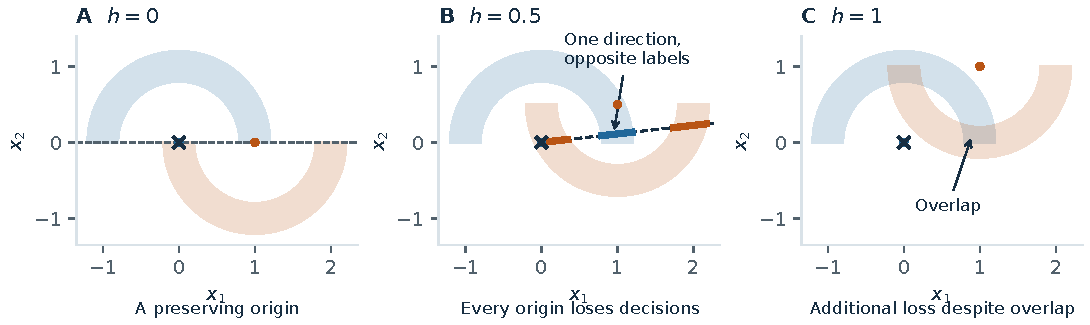
\includegraphics[width=\textwidth]{Fig1_Geometry.pdf}
\caption{Half-moon geometry and the effect of radial removal. Blue and orange indicate the two class supports; crosses mark the illustrated origin. The vertical displacement between class centers is $h$. (A) At $h=0$, the sign of the vertical direction preserves the label. (B) At $h=0.5$, one illustrated ray crosses both labels; the theorem establishes positive loss for every origin. Colored ray segments are exact support intersections. (C) At $h=1$, the original classes overlap, and normalization adds further ambiguity. The diagrams explain the mechanism; population risks are computed separately.}\label{fig:geometry}
\end{figure*}
\HalfMoonBackground
% Main-text fragment; supplementary proofs are in supplement_theory.tex.
% Requires amsmath, amssymb, booktabs and natbib.
\section{All-origin loss and computable Bayes risks}
\label{sec:origin-theory}

Direction-only normalization introduces unavoidable classification error throughout a disjoint half-moon family, and introduces additional error in the overlapping configuration. The result concerns every origin in the plane. We first express the lost decisions as cancellation along rays, then identify the geometry that forces this cancellation. A uniform projection limit closes the case of origins escaping to infinity, and signed-density cores make the global lower bound explicit. 

\begin{samepage}
Let $a=0.8$, $b=1.2$, $m_0=(0,0)$ and $m_1=(1,h)$, where $h$ is the upward center displacement. The open class supports are
\begin{align}
 S_0&=\{x:a<\|x\|<b,\ x_2>0\},\nonumber\\
 S_1&=\{x:a<\|x-m_1\|<b,\ x_2<h\}.
 \label{eq:halfmoon-supports}
\end{align}
\end{samepage}
Each support has area $H=\pi(b^2-a^2)/2=2\pi/5$. The primary generator has density $f_i^A=\mathbf1_{S_i}/H$; uniform radius and angle instead gives $f_i^R(x)=\mathbf1_{S_i}(x)/[\pi(b-a)\|x-m_i\|]$. The experiments use equal class priors. The geometric positivity results below hold for arbitrary positive priors $\pi_i$ and densities positive almost everywhere on their respective supports.

\paragraph{Decisions lost along a ray.}
Write $d=\pi_0f_0-\pi_1f_1$, $u_\theta=(\cos\theta,\sin\theta)$ and $[z]_+=\max(z,0)$. Positive $d$ favors class 0 and negative $d$ favors class 1 in the Bayes decision. Along a ray, the factor $r$ is the polar area Jacobian: a fixed angular slice covers more area at greater radius. Its positive and negative signed masses are
\begin{equation}
\begin{aligned}
 A_c(\theta)&=\int_0^\infty[d(c+ru_\theta)]_+r\,dr,\\
 B_c(\theta)&=\int_0^\infty[-d(c+ru_\theta)]_+r\,dr.
\end{aligned}
\label{eq:ray-masses-main}
\end{equation}
Let $R_X^*$ and $R^*_{T_c}$ denote the minimum classification risks from raw coordinates and directions, respectively. Using the masses in~\eqref{eq:ray-masses-main}, the binary Bayes-risk identity yields
\begin{equation}
 \Delta(c):=R^*_{T_c}-R_X^*
 =\int_0^{2\pi}\min\{A_c(\theta),B_c(\theta)\}\,d\theta.
 \label{eq:ray-loss-main}
\end{equation}
Each minimum counts the smaller opposing decision mass merged on that ray. Loss is positive exactly when a positive-measure set of rays combines opposite Bayes preferences. This specializes the established decision-preservation framework \citep{Silva2012,Silva2024} to the origin-dependent direction map. Supplementary Section~\ref{supp:bayes} derives the identity.

\paragraph{Theorem 1: an all-origin transition.}
For $0<h\leq\sqrt{3/5}$, the supports have disjoint interiors and
\begin{equation}
 R_X^*=0,\qquad \Delta(c)>0
 \quad\text{for every }c\in\mathbb R^2.
 \label{eq:all-origin-disjoint}
\end{equation}
At $h=0$, every origin with $c_2=0$ preserves zero risk. More generally, for $h<0$, origins in the separating strip $h\leq c_2\leq0$ preserve zero risk. At $h=1$, the supports overlap and
\begin{equation}
 R_X^*>0,\qquad \Delta(c)>0
 \quad\text{for every }c\in\mathbb R^2.
 \label{eq:all-origin-overlap}
\end{equation}

\emph{Proof sketch.}
For $0\leq h\leq a$, horizontal slicing reduces disjointness to
$\sqrt{a^2-h^2}\geq1/5$, giving the stated threshold. Throughout its positive range, the connected supports intrude into each other's convex hull: $(1,h/2)\in S_0\cap\operatorname{int}\operatorname{conv}(S_1)$ and its reflection belongs to the reverse intersection. The relevant geometric criterion is a probabilistic adaptation of the separability geometry of Hurtado et al.\ \citep{Hurtado2001}. Two connected open regions with mutual convex-hull intrusion have overlapping direction images from every origin. Indeed, disjoint images would be open arcs, at least one of length at most $\pi$; the convex cone generated by that arc would contain its region's convex hull and exclude the other region. Positive densities turn the resulting open angular overlap into positive loss in~\eqref{eq:ray-loss-main}.

For $h=1$, the same argument applies to connected regions exclusive to each class. One class has a connected backbone through $(1,1/4)$, $(-1,1/20)$ and $(0,11/10)$, with a radius-$1/20$ neighborhood contained in its exclusive region. Reflection about $(1/2,1/2)$ produces the other backbone. Strictly positive barycentric coordinates establish mutual hull intrusion. This forces additional loss even though the raw classes already overlap. Supplementary Sections~\ref{supp:geometry}--\ref{supp:overlap} give the complete constructions and proofs.

% Suggested main-text replacement/extension for the old positive-infimum theorem.
% The supplement fragment defines supp:projection-boundary.
\paragraph{Theorem 2: the decision problem at distant origins.}
A positive loss at each fixed origin can still approach zero along an unbounded sequence of origins. To determine a global floor, we also control these escaping sequences. Moving the origin far from the data makes its rays almost parallel. Orthogonal projections are the geometric boundary of radial projections \citep{Orponen2019}; the following result identifies their classification-risk limit. It applies to binary populations with densities in any dimension $n\geq2$. Fix a reference point $p$, let $e$ be a unit vector, and let $P_e$ project onto the hyperplane perpendicular to $e$. Then
\begin{equation}
 \lim_{R\to\infty}\sup_e
 \left|R^*_{T_{p+Re}}-R^*_{P_e}\right|=0.
 \label{eq:projection-limit-main}
\end{equation}
Write $\Delta_\infty(e)=R^*_{P_e}-R_X^*$. The loss surface, completed by these projection limits, is continuous on a compact domain. Consequently,
\begin{equation}
 \inf_c\Delta(c)>0
 \quad\Longleftrightarrow\quad
 \begin{cases}
 \Delta(c)>0&\text{all finite }c,\\
 \Delta_\infty(e)>0&\text{all directions }e.
 \end{cases}
 \label{eq:global-criterion-main}
\end{equation}
Thus optimizing the origin cannot make loss vanish when both finite radial views and all limiting linear projections lose decisions.

\emph{Half-moon consequence.}
The connected winner regions in Theorem~1 have overlapping projection intervals in every direction. Equations~\eqref{eq:projection-limit-main}--\eqref{eq:global-criterion-main} therefore strengthen its conclusion to
\begin{equation}
 \inf_{c\in\mathbb R^2}\Delta(c)>0
 \quad\text{for }0<h\leq\sqrt{3/5}\text{ and for }h=1.
 \label{eq:global-positive}
\end{equation}
This holds for every fixed pair of positive priors and densities positive almost everywhere on their respective supports. The proof controls signed probability mass in total variation, so it establishes convergence of the optimal decision risk. Supplementary Section~\ref{supp:projection-boundary} proves the general result and gives an explicit convergence bound for bounded-support densities of bounded variation.

% Standalone main-text replacement paragraph. Definitions of d and Delta precede it.
\paragraph{A constructive certificate over all origins.}
The loss floor can be bounded using regions where the preferred class has a fixed probability margin. In the plane, let $K_+,K_-$ be compact connected cores whose radius-$\rho$ neighborhoods satisfy $d\geq\kappa_+>0$ and $d\leq-\kappa_-<0$, respectively. Suppose each core meets the other's convex hull, their convex hulls contain a common disk $B(p,\delta)$, and both cores lie within distance $M$ of $p$. Writing $\kappa=\min(\kappa_+,\kappa_-)$ gives
\begin{equation}
 \inf_c\Delta(c)\geq\kappa\min\left\{
 \frac{\sqrt3\rho^3}{6M},\;2\rho\delta\right\}>0.
 \label{eq:constructive-global}
\end{equation}
For bounded origins, mutual hull intrusion supplies a ray through both cores. Their neighborhoods give a common angular interval carrying a fixed amount of opposing signed mass. For exterior origins, rays through the common hull disk supply the bound. Supplementary Section~\ref{supp:constructive-global} proves the result and optimizes the split between these regions. For equal-prior area sampling, optimized whole-plane lower certificates exceed $0.0205$ percentage points (pp) at $h=0.5$ and $0.00119$~pp at $h=1$. Eroded half-annuli provide such cores throughout the disjoint regime of Theorem~1 under both sampling laws and any fixed positive priors.

\paragraph{Fixed-origin risk calculation.}
For the half-annuli, circle tangencies and boundary intersections partition directions into finitely many cells. Radial support order is fixed inside a cell, so one representative ray determines whether opposite preferences coexist. Exact radial primitives then reduce Bayes risk to one angular integral. Ball arithmetic and a bounded-variation truncation bound certify its value. Supplementary Sections~\ref{supp:finite}--\ref{supp:bv} give the finite preservation test, integration formulas and error bounds. At equal priors, the density ratio $f_i^R/f_i^A\in[5/6,5/4]$ also gives $\Delta_R(c)\geq(5/6)\Delta_A(c)$.

\paragraph{One bit repairs the disjoint midpoint representation.}
At $h=0.5$, direction alone has positive loss at every origin. At the midpoint $c=(1/2,1/4)$, append the single radial bit $q=\mathbf1\{\|x-c\|>4/5\}$. For $q=0$, the sign of $9u_1+10u_2$ determines the class; for $q=1$, the sign of $u_2-u_1$ determines it. Positive signs identify class~0. Figure~\ref{fig:bit-repair} shows how the radial bit assigns observations to the two angular rules. Together, the two rules correctly label the complete class supports under their respective bit conditions, giving zero Bayes risk under either sampling law and any positive priors. Supplementary Section~\ref{supp:one-bit} proves the separating inequalities. Since zero additional radial bits leave the positive direction-only floor, one bit is the minimal radial addition at this geometry.

\paragraph{Certified thresholds and radius-error tolerance.}
With the same angular rules, recovery is exact precisely for $\alpha\leq t\leq\beta$, where $\alpha\approx0.7433034374$ and $\beta\approx0.8120914734$ (Threshold Addendum, Proposition~1). If the measured radius is $\widehat r=r+e$, $|e|\leq\varepsilon$, every support label is preserved for every admissible error function exactly when
\begin{equation}
\alpha+\varepsilon\leq t\leq\beta-\varepsilon.
\label{eq:radius-error}
\end{equation}
The midpoint threshold $t_\star=(\alpha+\beta)/2\approx0.7776974554$ maximizes the guaranteed tolerance at $(\beta-\alpha)/2\approx0.0343940180$ (Addendum, Corollary~1). The neural experiments retain $t=0.8$.

\begin{figure*}[t]
\centering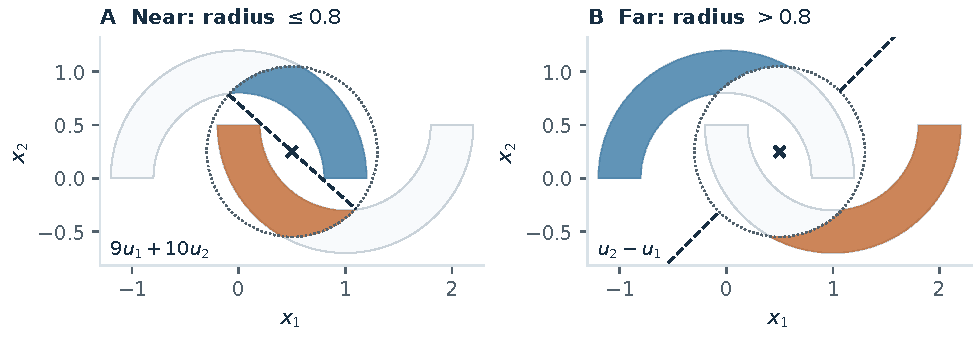
\includegraphics[width=.84\textwidth]{Fig2_One_Bit_Recovery.pdf}
\caption{Exact one-bit recovery at $h=0.5$. The same radius threshold, $0.8$ about $c=(0.5,0.25)$, applies to every direction. (A) Inside the threshold, $9u_1+10u_2$ separates the two classes. (B) Outside it, $u_2-u_1$ separates them. Blue denotes class 0 and orange class 1. Each panel shows the portion of the original supports assigned to that radial code; the dashed line is its angular decision boundary. Direction together with the bit determines the class.}\label{fig:bit-repair}
\end{figure*}
% Experimental sections drawn only from the frozen and audited neural study.
% Requires booktabs and natbib. Add experimental_references.bib to the bibliography.
% Invoke \HalfMoonExperiments in the main text; place
% \HalfMoonExperimentalLimitations inside the consolidated limitations section.

\newcommand{\HalfMoonExperiments}{%
\section{Controlled neural experiments}
\label{sec:experiments}

\subsection{Design and evaluation}
We tested whether learned errors track the origin-dependent population risks. Equal-prior observations were sampled uniformly in area from half-annuli with radii $0.8$ and $1.2$, centered at $(0,0)$ and $(1,h)$, for $h\in\{-0.25,0.5,1\}$. Each of ten independent dataset/initialization seeds, numbered 1001--1010, supplied balanced training, validation and test sets of 2,000, 2,000 and 50,000 observations. Within each geometry/seed, conditions shared observations; initializations were paired across conditions and geometries. Data-generation phases, geometries and splits used distinct streams.

The five inputs were raw coordinates $R$; directions $D_0$, $D_M$ and $D_A$ about $(0,0)$, $(0.5,h/2)$ and $(0,3)$; and $P_A$, which retained direction and radius about $(0,3)$. Direction used exact division by the nonzero norm, with zero residual mapped to zero. After transformation, features were standardized using their training mean and population standard deviation; exactly constant features used scale one. This positive affine transformation preserves the representation's information.

The principal network comprised 64 tanh hidden units and a linear output. We fitted labels $-1/+1$ by mean squared error (MSE), assigning positive outputs to the second class. Full-batch Adam~\citep{Kingma2015} used $(\beta_1,\beta_2)=(0.9,0.999)$, optimizer $\epsilon=10^{-8}$, and learning rates $0.001$ and $0.01$. Every candidate executed 4,000 updates.\footnote{The stopping criterion was completion of the fixed update budget, including candidates whose selected checkpoint occurred earlier.} Validation was evaluated at initialization and every 50 updates. Selection minimized validation error, followed by validation MSE, earlier update and lower learning rate.

The main design required 300 candidate fits. At $h=1$, width-15 and unconditioned width-64 diagnostics each added 60 fits for $R,D_A,P_A$. These 420 final candidate fits were separate from a 48-fit development stage using seeds 101 and 103. Training and analysis protocols were frozen before final test generation; the 210 selected models were then evaluated once. 

Misclassification error was the primary outcome; accuracy, MSE and error above the applicable Bayes floor were secondary. Six prespecified paired contrasts compared $D_M-D_0$ and $D_A-D_0$ at each $h$. The dataset/initialization seed was the inference unit. We summarized paired seed differences using their mean, sample standard deviation and Student-$t$ intervals with nine degrees of freedom. Simultaneous 95\% intervals used $t_9(1-0.05/12)$ for the six-contrast family. Supplementary results retain whole-seed bootstrap sensitivity analyses and pointwise diagnostic intervals.

The analytical Bayes rule was evaluated on the identical test observations. Class-specific errors and class-stratified Monte Carlo standard errors separated test sampling from numerical integration bounds and between-seed variation. Across the 15 main conditions, mean empirical Bayes-rule error differed from integrated risk by at most $0.061$ percentage points (pp).

\subsection{Results}
Learned errors approached their representation-specific floors: the largest mean excess among the 15 main conditions was $0.471$~pp (Table~\ref{tab:neural-main}). For $h=0.5$, raw and direction-plus-radius inputs produced zero observed test errors, whereas all three direction-only inputs incurred errors consistent with their positive population floors. At $h=1$, $R$ and $P_A$ achieved $6.790\%$ and $6.833\%$ error against their common $6.716\%$ floor.

All five nonzero primary origin contrasts had simultaneous intervals excluding zero (Supplementary Table~\ref{tab:neural-contrasts}). The midpoint reduced error relative to the zero origin in both nonlinear configurations. The upper origin increased error by $9.379$~pp at $h=0.5$ and decreased it by $1.445$~pp at $h=1$. For $h=-0.25$, $D_M-D_0$ was zero for every seed. Thus the effect of changing origin followed the class arrangement.

The paired $P_A-R$ difference at $h=1$ was $0.044$~pp, with a pointwise 95\% interval $[-0.043,0.130]$. All three width-15 versus width-64 diagnostic intervals included zero. Removing affine conditioning increased $D_A$ error by $0.179$~pp, $[0.053,0.305]$; the corresponding $R$ and $P_A$ intervals included zero. Complete seed outcomes, signed excess estimates, prediction arrays and learning histories accompany the experiment.

\HalfMoonMainRiskTable

}

\newcommand{\HalfMoonMainRiskTable}{%
\begin{table}[t]
\centering\small
\setlength{\tabcolsep}{3pt}
\caption{Population Bayes risk and neural test error. Errors are mean $\pm$ sample SD over ten seeds; excess is mean error minus Bayes risk. Risk and error are percentages; excess is in percentage points. $R$ denotes raw coordinates, $D$ direction, and $P$ direction plus radius; subscripts $0$, $M$ and $A$ identify the zero, midpoint and upper origins.}
\label{tab:neural-main}
\begin{tabular}{rrrcr}
\toprule
$h$ & Input & Bayes risk & Test error & Excess \\
\midrule
$-0.25$ & $R$   & 0.0000 & $0.000\pm0.000$ & 0.000 \\
         & $D_0$ & 0.0000 & $0.000\pm0.000$ & 0.000 \\
         & $D_M$ & 0.0000 & $0.000\pm0.000$ & 0.000 \\
         & $D_A$ & 22.2934 & $22.528\pm0.176$ & 0.234 \\
         & $P_A$ & 0.0000 & $0.000\pm0.000$ & 0.000 \\
\addlinespace
$0.5$    & $R$   & 0.0000 & $0.000\pm0.000$ & 0.000 \\
         & $D_0$ & 11.8577 & $11.991\pm0.132$ & 0.134 \\
         & $D_M$ & 10.7479 & $10.835\pm0.140$ & 0.087 \\
         & $D_A$ & 21.1509 & $21.370\pm0.268$ & 0.219 \\
         & $P_A$ & 0.0000 & $0.000\pm0.000$ & 0.000 \\
\addlinespace
$1$      & $R$   & 6.7157 & $6.790\pm0.103$ & 0.074 \\
         & $D_0$ & 21.7294 & $22.201\pm0.375$ & 0.471 \\
         & $D_M$ & 20.8548 & $20.947\pm0.175$ & 0.092 \\
         & $D_A$ & 20.5987 & $20.755\pm0.316$ & 0.157 \\
         & $P_A$ & 6.7157 & $6.833\pm0.135$ & 0.118 \\
\bottomrule
\end{tabular}
\end{table}
}

\newcommand{\HalfMoonOriginContrastTable}{%
\begin{table}[t]
\centering\small
\setlength{\tabcolsep}{3pt}
\caption{Prespecified origin contrasts in percentage points. Intervals are simultaneous 95\% Bonferroni-adjusted paired-$t$ intervals for all six comparisons.}
\label{tab:neural-contrasts}
\begin{tabular}{rlrl}
\toprule
$h$ & Contrast & Mean & Simultaneous interval \\
\midrule
$-0.25$ & $D_M-D_0$ & 0.000 & $[0.000,0.000]$ \\
         & $D_A-D_0$ & 22.528 & $[22.341,22.715]$ \\
$0.5$    & $D_M-D_0$ & $-1.156$ & $[-1.292,-1.020]$ \\
         & $D_A-D_0$ & 9.379 & $[9.083,9.675]$ \\
$1$      & $D_M-D_0$ & $-1.254$ & $[-1.755,-0.752]$ \\
         & $D_A-D_0$ & $-1.445$ & $[-1.879,-1.012]$ \\
\bottomrule
\end{tabular}
\end{table}
}

% Place this macro only in the consolidated limitations section.
\newcommand{\HalfMoonExperimentalLimitations}{%
The neural evidence covers three area-uniform, equal-prior populations, ten dataset/initialization seeds and the stated single-hidden-layer training budget. Error above a representation's floor combines approximation, optimization and finite-training-sample effects. The density-sensitivity analysis concerns population risks. The capacity and conditioning intervals describe their prespecified diagnostic comparisons.
}

\HalfMoonExperiments
\subsection{Independent test of the one-bit repair}
\label{sec:one-bit-experiment}
We tested the constructive repair at $h=0.5$ with ten fresh paired dataset/initialization seeds (2001--2010). The four inputs were $R$, midpoint direction $D_M$, midpoint direction with the bit $q$ ($B$), and midpoint direction with the full radius ($P_M$). The bit threshold $0.8$ was fixed by the geometric construction before this experiment. The same sample sizes, 64-unit architecture, two learning rates, 4,000-update budget, conditioning and validation selection rule were retained. The 80 new candidate fits produced 40 selected models; their test sets used an independent random namespace and were evaluated after selection was frozen. The paired contrasts $B-D_M$ and $B-P_M$ formed a separate two-comparison family with simultaneous 95\% Bonferroni-adjusted intervals. $B$ and $P_M$ each used three inputs and 321 parameters; $R$ and $D_M$ used two inputs and 257 parameters.

The one-bit networks made three errors across 500,000 test observations, compared with 54,362 errors for direction alone (Table~\ref{tab:one-bit-neural}). The mean $B-D_M$ difference was $-10.8718$~pp. Its simultaneous 95\% confidence interval was $[-10.9691,-10.7745]$. The $B-P_M$ difference was $0.0006$~pp, $[-0.0010,0.0022]$. Raw and full-radius networks made no observed errors. The explicit decoder also classified all 500,000 observations correctly. Supplementary Section~\ref{supp:one-bit-experiment} reports seed outcomes and bootstrap sensitivity results.

\begin{table}[t]
\centering\small
\setlength{\tabcolsep}{3pt}
\caption{Fresh one-bit experiment at $h=0.5$. Bayes risk and mean $\pm$ sample SD over ten seeds are percentages. Each input is evaluated on the same 500,000 observations, balanced within each seed. $R$ denotes raw coordinates; $D_M$, midpoint direction; $B$, midpoint direction plus one bit; and $P_M$, midpoint direction plus full radius.}
\label{tab:one-bit-neural}
\begin{tabular}{lrrr}
\toprule
Input & Bayes risk & Test error & Error count \\
\midrule
$R$ & 0 & $0.0000\pm0.0000$ & 0 \\
$D_M$ & 10.7479 & $10.8724\pm0.1157$ & 54,362 \\
$B$ & 0 & $0.0006\pm0.0019$ & 3 \\
$P_M$ & 0 & $0.0000\pm0.0000$ & 0 \\
\bottomrule
\end{tabular}
\end{table}

\HalfMoonDiscussion
\subsection{Limitations}
The half-moon results use two-dimensional half-annular supports and exact direction normalization. The general projection-limit theorem covers absolutely continuous binary populations; the explicit global certificates require connected signed-density cores and are conservative lower bounds. The one-bit construction, fixed-decoder threshold interval and radius-error guarantee use $h=0.5$, the fixed midpoint and exact direction. Neural inference uses ten replicates per experiment, equal priors, area-uniform sampling and one hidden-layer learner with a fixed training budget. The radius-uniform comparison concerns population risks. Learned excess combines finite-sample, approximation and optimization effects.
\section{Conclusion}
Changing the normalization origin cannot eliminate classification loss for the proved half-moon configurations. The distant-origin limit and signed-density certificates establish this claim over the entire origin plane. At $h=0.5$, one common-threshold radius bit restores zero Bayes risk over a certified operating interval and achieves the minimum additional radial budget. The same interval determines the largest bounded radius error the fixed decoder tolerates and the threshold maximizing that tolerance. The paired neural studies measure how learned errors relate to these population limits. Together, the results provide a way to diagnose loss before classifier training and to retain precisely the radial information needed for recovery in the constructed geometry.
\section*{Data availability}
The generators, frozen protocols, numerical certificates, trained weights, predictions and analysis code are available in the \href{https://github.com/Meshaal-Mouawad/HalfMoon-Direction-Normalization/releases/tag/v11-submission}{public V11 research release}. The archive includes the Threshold Addendum and reproducible checks for the threshold interval and radius-error guarantee.
\section*{Declaration of generative AI and AI-assisted technologies in the preparation process}
During preparation of this work, the author used Elsevier LeapSpace and other tools to support literature discovery, manuscript organization, language refinement, and consistency checking. The author takes responsibility for the content of the article.
\bibliographystyle{unsrtnat}
\bibliography{references}
\end{document}
